% !TeX root = RJwrapper_eng.tex
\title{WLinfer: Statistical Inference for Weighted Lindley Distribution}
\author{by Yu-Hyeong Jang, SungBum Kim, Hyun-Ju Jung, and Hyoung-Moon Kim}

\maketitle

\abstract{
	New distributions are still being suggested for better  fitting of a distribution to data, as it is one of the most fundamental problems in terms of the parametric approach. One of such is weighted Lindley (WL) distribution \citep{ghitany:2011}. Even though WL distribution has become increasingly popular as a possible alternative to traditional distributions such as gamma and log normal distributions, fitting it to data has rarely been addressed in existing R packages. This is the reason we present the \CRANpkg{WLinfer} package that implements overall statistical inference for WL distribution. In particular, \pkg{WLinfer} enables one to conduct the goodness of fit test, point estimation, bias correction, interval estimation, and the likelihood ratio test simply with the \samp{WL} function which is at the core of this package. To assist users who are unfamiliar with WL distribution, we present a brief review followed by an illustrative example with R codes.
}

\section{Introduction}

Weighted Lindley (WL) distribution has recently received considerable attention since it provides a more flexible fit to data from various fields than traditional widely-used distributions such as exponential, log normal, and gamma distributions \citep{ghitany:2011,mazucheli:2013}.
The probability density function (pdf) of WL distribution is given by
\begin{equation*}
f(x) = \frac{\lambda^{\phi+1}}{(\lambda+\phi)\Gamma(\phi)}{x}^{\phi-1}(1+{x})\exp(-\lambda {x}),
\hspace{6pt}x>0,\lambda>0,\phi>0,
\end{equation*} 
which can be interpreted as a mixture of two gamma distributions
\begin{equation*}
\begin{aligned}
&f(x) = \frac{\lambda}{\lambda+\phi}f_{1}(x)+\frac{\phi}{\lambda+\phi}f_{2}(x),\quad x>0,\lambda>0,\phi>0,
\end{aligned}
\end{equation*}
where
\begin{equation*}
\begin{aligned}
&f_{i}(x) = \frac{\lambda^{\phi+i-1}}{\Gamma(\phi+i-1)}x^{\phi+i-2} \exp (-\lambda x),\quad x>0,\lambda>0,\phi>0,\quad i=1,2.
\end{aligned}
\end{equation*}  
Due to its nature as a gamma mixture, however, statistical inference for WL distribution, such as parameter estimation, bias correction, interval estimation, and statistical test, is overall more cumbersome and tedious than those of the aforementioned distributions. 

Despite this difficulty, there is no existing R package that implements this comprehensive process for WL distribution. To the best of our knowledge, \CRANpkg{mle.tools} \citep{mtools:2017} is the only R package that enables one to obtain maximum likelihood (ML) estimates for WL distribution with  asymptotic variance and bias correction. However, they are just limited to ML estimates. An R package \CRANpkg{fitdistrplus} \citep{fitdistrplus:2015} which fits certain univariate distributions to data sets is not applicable to WL distribution, while  \CRANpkg{LindleyR} package \citep{lindleyr} is exclusively for the use of pdf, cumulative distribution function (cdf), quantile, and random number generation, not statistical inference itself.

Based on this motivation, we present an R package \CRANpkg{WLinfer} by providing various estimation methods in addition to maximum likelihood estimator (MLE), such as  method of moment estimator (MME), modified method of moment estimator (MME$_m$), and closed form MLE-like estimator (MLE$_c$). For bias correction, \pkg{WLinfer} encompasses Firth's method and the bootstrap method which were not considered in \pkg{mle.tools}, as well as Cox and Snell's method. Furthermore, \pkg{WLinfer} provides the goodness of fit and likelihood ratio tests.

The remainder of this paper is organized as follows. First, we briefly review the theoretical results for each inferential step ranging from the goodness of fit test to the likelihood ratio test, while introducing relevant arguments of the \samp{WL} function. We then provide an example to illustrate the whole output of \samp{WL} function and how to use \samp{WL} function which implements the whole statistical inference at once. Finally, we conclude with summarizing remarks.

The \pkg{WLinfer} package is available from the Comprehensive R Archive Network (CRAN) at \url{https://CRAN.R-project.org/package=WLinfer}. R code for the examples demonstrated herein has been provided as supplementary material. The supplementary code has been tested with \pkg{WLinfer} version 1.0.0, and results presented herein have been produced with this version.





\section{Goodness of fit test}
The first step in fitting a distribution to data is to check whether the data can be assumed as generated from the distribution. For this purpose, many goodness of fit tests have been developed. Among them, \pkg{WLinfer} includes three popular tests: the Kolmogorov-Smirnov test, the Anderson-Darling test, and the Cramér-von Mises test. Uncertainty that could occur from using estimates instead of true values are not considered here. The argument \code{dist$\_$test} of \samp{WL} function is specified by one of either \code{"ks"}, \code{"cvm"}, \code{"ad"}, or \code{"all"}. The default is \code{dist$\_$test="ks"} while \code{dist$\_$test=all"} returns the results of all three tests.





\section{Point estimation}
\pkg{WLinfer} package considers four estimators: MLE, MLE$_{c}$, MME and MME$_{m}$. To the best of our knowledge, these are the only estimators of which asymptotic distribution has been analytically proven. In this study, we only review the estimation formulas. Please refer to \cite{kim:2020,ghitany:2017,mazucheli:2013} for more specific theoretical results.
\begin{itemize}
	\item[$\bullet$] 
	MLE of WL distribution is obtained by
	$$
	\widehat{\lambda}_{MLE}=\frac{-\widehat{\phi}_{MLE}(\overline{X}-1)+\sqrt{\left[\widehat{\phi}_{MLE}(\overline{X}-1)\right]^{2}+4 \widehat{\phi}_{MLE}\left(\widehat{\phi}_{MLE}+1\right) \overline{X}}}{2 \overline{X}}
	$$
	where $\widehat{\phi}_{MLE}$ is the solution of the nonlinear equation
	$$
	\psi\left(\widehat{\phi}_{MLE}\right)+\frac{1}{\widehat{\lambda}_{MLE}+\widehat{\phi}_{MLE}}- \log \left( \widehat{\lambda}_{MLE} \right) - \frac{1}{n} \sum_{i=1}^{n} \log \left(x_{i}\right)=0,$$
	with $\psi(x)= \cfrac{\mathrm{d}\log\ ( \Gamma(x))}{\mathrm{d} x}$.
	\\
	\item[$\bullet$] MLE$_{c}$\\
	$\begin{array}{l}
	\widehat{\lambda}_{MLE_c}=    \cfrac{d +\sqrt{d^2 +  \frac{4(1+a_1)\cdot a_0 (a_0 - 1)  }{\left(\sum X_{i} / n\right)-a_1}}}{2(a_1+1)},     \label{eq:ClosedFormLambda} \quad\quad
	\widehat{\phi}_{MLE_c}= a_1 \widehat{\lambda}- a_0,\label{eq:ClosedFormPhi}
	\end{array}$ \\
	where 
	$\begin{array}{l}
	d = a_0 +\frac{(1+a_1 )(1-a_0 )-1}{\sum X_{i}/n-a_1 }, \quad
	a_1 = \cfrac{\sum\limits_{i}^{n} X_{i} \log (X_{i})}{\sum\limits_{i}^{n} \log (X_{i})}~ \text{and}~ 
	a_0 = \cfrac{\sum\limits_{i}^{n} \frac{X_{i} \log (X_{i})}{1+X_{i}}+n }{\sum\limits_{i}^{n} \log (X_{i})}.
	\end{array}$
	\\
	\item[$\bullet$] MME\\
	$\begin{array}{l}
	\widehat{\lambda}_{MME}=\cfrac{-\widehat{\phi}_{MME}(\overline{X}-1)+\sqrt{\left[\widehat{\phi}_{MME}(\overline{X}-1)\right]^{2}+4 \overline{X} \widehat{\phi}_{MME}\left(\widehat{\phi}_{MME}+1\right)}}{2 \overline{X}}, \\
	\\
	\widehat{\phi}_{MME}=\cfrac{- g \left(\overline{X}, S^{2}\right)+\sqrt{\left[g \left(\overline{X}, S^{2}\right)\right]^{2}+16 S^{2}\left[S^{2}+(\overline{X}+1)^{2}\right] \overline{X}^{3}}}{2 S^{2}\left[S^{2}+(\overline{X}+1)^{2}\right]},\\
	\text{where } g \left(\overline{X}, S^{2}\right)=S^{4}-\overline{X}\left(\overline{X}^{3}+2 \overline{X}^{2}+\overline{X}-4 S^{2}\right),\quad S^{2}=\frac{1}{n} \sum_{i=1}^{n}\left(X_{i}-\overline{X}\right)^{2}.
	\end{array}$
	\\
	\item[$\bullet$] MME$_{m}$\\
	$	\begin{array}{l}
	\widehat{\lambda}_{MME_{m}}=\cfrac{\overline{X^*}(1-\overline{X^{*}})}{\overline{X}\cdot \overline{X^{*}}-(1-\overline{X^{*}})}, \\ \widehat{\phi}_{MME_{m}}=\cfrac{(1-\overline{X^{*}})^{2}}{\overline{X}\cdot \overline{X^{*}}-(1-\overline{X^{*}})},\quad\text{where } X^{*}=\cfrac{1}{1+X}.
	\end{array}$
\end{itemize}
Each estimation method can be implemented by choosing \samp{est$\_$method} of \samp{WL} function, among \code{"MLE"}, \code{"MLEc"}, \code{"MME"}, and \code{"MMEm"}. The default refers to \samp{est$\_$method = "MLEc"}.
If point estimation is solely of interest, one can separately obtain point estimates with the following codes:
\begin{example}
	data(fail_fiber)  # fail_fiber is included in WLinfer package.
	
	MLEc_WL(fail_fiber)  # Closed form MLE-like estimator
	MME_WL(fail_fiber)  # Method of moment estimator
	MMEm_WL(fail_fiber)  # Modified method of moment estimator
	MLE_WL(fail_fiber,init =1)  # Initial value for phi is required.
\end{example}
We use \code{fail$\_$fiber} data set \citep{bader:1982} which is included in the \pkg{WLinfer} package. This data set consists of 65 observations of the strength measurement of carbon fiber.






\section{Bias correction}
Unless sample size is sufficient for achieving consistency, bias correction is highly recommended since all the aforementioned estimators are upwardly biased in the case of small samples \citep{kim:2020,mazucheli:2013,wang:2017}. To this end, the \pkg{WLinfer} package provides three bias correction methods: Cox and Snell's method \citep{cox:1968,cordeir:1994} for MLE and MLE$_c$, Firth's method \citep{firth:1993} for MLE, and the bootstrap method \citep{efron:1979,efron:1986} for MLE$_c$. After a series of tedious calculations, correction formulas are given as follows: 

\begin{itemize}
	\item[$\bullet$] Cox and Snell's method \\
	$\widehat{\boldsymbol\theta}_{CMLE}=\widehat{\boldsymbol{\theta}}_{M L E}-\left(\begin{array}{c}
	\delta(\widehat{\lambda}) \\
	\delta(\widehat{\phi})
	\end{array}\right),$ \\
	%=\widehat{\boldsymbol\theta}_{MLE}-\widehat{K}^{-1} \widehat{A} %\operatorname{vec}\left(\widehat{K}^{-1}\right)\big\rvert_{\boldsymbol\theta=%\widehat{\boldsymbol\theta}_{MLE}}
	$\widehat{\boldsymbol\theta}_{CMLE_{c}}=\widehat{\boldsymbol{\theta}}_{M L E_{c}}-\left(\begin{array}{c}
	\delta(\widehat{\lambda}) \\
	\delta(\widehat{\phi})
	\end{array}\right),$ \\
	%=\widehat{\boldsymbol\theta}_{MLE_{c}}-\widehat{K}^{-1} \widehat{A} %\operatorname{vec}\left(\widehat{K}^{-1}\right)\big\rvert_{\boldsymbol\theta=%\widehat{\boldsymbol\theta}_{MLE_{c}}}
	where
	$\delta(\widehat{\lambda}) =  \cfrac{1}{n}\cdot \frac{ N_{1} \big\rvert_{\boldsymbol\theta=\widehat{\boldsymbol\theta}_{MLE_{c}s}}}{D \big\rvert_{\boldsymbol\theta=\widehat{\boldsymbol\theta}_{MLE_{c}s}}} ~\text{and}~
	\delta(\widehat{\phi}) = \cfrac{1}{n}\cdot \frac{ N_{2} \big\rvert_{\boldsymbol\theta=\widehat{\boldsymbol\theta}_{MLE_{c}s}} }{D \big\rvert_{\boldsymbol\theta=\widehat{\boldsymbol\theta}_{MLE_{c}s}}}$ 
	with\\
	$\begin{aligned}
	D =& \left[ \left( \psi^{\prime} (\phi) - \frac{1}{(\lambda+ \phi)^2} \right)  \left( \frac{\phi+1}{\lambda^2} - \frac{1}{(\lambda+\phi)^2}  \right) - \left( \frac{1}{(\lambda+\phi)^2} + \frac{1}{\lambda}  \right)^2 \right]^2,\\
	\end{aligned}$
	
	$\begin{aligned}
	N_{1} =& \left( \frac{1}{(\lambda+\phi)^2} - \psi' (\phi)  \right) \left[ \left( \frac{1}{(\lambda+\phi)^2} - \psi' (\phi)  \right) \left(  \frac{\phi + 1}{\lambda^3} - \frac{1}{(\lambda+ \phi)^3} \right) + \left( \frac{1}{\lambda} + \frac{1}{(\lambda + \phi)^2} \right) \left( \frac{1}{2 \lambda^2} + \frac{1}{(\lambda+\phi)^3} \right) \right]\\
	&+ 2 \left( \frac{1}{\lambda} + \frac{1}{(\lambda+\phi)^2} \right) \left[ \left( \frac{1}{(\lambda+\phi)^2} - \psi' (\phi) \right) \left( \frac{1}{2 \lambda^2} + \frac{1}{(\lambda + \phi)^3}   \right)  - \left( \frac{1}{\lambda} + \frac{1}{(\lambda + \phi)^2} \right) \frac{1}{(\lambda + \phi)^3} \right] \\
	&+ \left( \frac{1}{(\lambda + \phi)^2} - \frac{\phi + 1}{\lambda^2} \right) \left[ \left( \psi' (\phi) - \frac{1}{(\lambda+\phi)^2} \right) \frac{1}{(\lambda + \phi)^3} + \left( \frac{1}{\lambda} + \frac{1}{(\lambda + \phi)^2}  \right) \left( \frac{1}{(\lambda + \phi)^3} +\frac{\psi'' (\phi)}{2} \right)  \right],\\
	\end{aligned}$
	
	$\begin{aligned}
	N_{2} =&  \left( \frac{1}{(\lambda + \phi)^2} - \psi' (\phi) \right) \left[ \left(   \frac{\phi+1}{\lambda^2} - \frac{1}{(\lambda + \phi)^2} \right) \left( \frac{1}{2 \lambda^2} + \frac{1}{(\lambda + \phi)^3}  \right) + \left( \frac{1}{\lambda} + \frac{1}{(\lambda + \phi)^2} \right)  \left( \frac{1}{(\lambda + \phi)^3} - \frac{\phi+1}{\lambda^3}  \right) \right] \\
	&- 2 \left( \frac{1}{\lambda} + \frac{1}{(\lambda + \phi)^2}  \right) \left[ \left( \frac{1}{\lambda} + \frac{1}{(\lambda + \phi)^2} \right) \left( \frac{1}{2 \lambda^2} + \frac{1}{( \lambda + \phi)^3} \right) + \left( \frac{\phi+1}{\lambda^2} - \frac{1}{(\lambda + \phi)^2} \right) \frac{1}{(\lambda + \phi)^3}  \right]\\
	&+ \left( \frac{\phi+1}{\lambda^2} - \frac{1}{(\lambda+ \phi)^2}  \right) \left[ \left( \frac{1}{(\lambda +\phi)^2} - \frac{\phi+1}{\lambda^2} \right)  \left( \frac{1}{(\lambda + \phi)^3} + \frac{\psi'' (\phi)}{2} \right)  - \left( \frac{1}{\lambda} + \frac{1}{(\lambda+\phi)^2} \right) \frac{1}{(\lambda + \phi)^3} \right].
	\end{aligned}$\\
	
	\item[$\bullet$] Firth's method \\
	The estimator corrected by Firth's method is obtained by solving modified likelihood equations given by
	$$ \left(\begin{array}{l}
	\partial l / \partial \lambda \\
	\partial l / \partial \phi
	\end{array}\right)-A \operatorname{vec}\left(K^{-1}\right)=\boldsymbol{0}, $$
	where\\
	$\begin{aligned}
	A &= n\left[\begin{array}{cccc}
	\frac{\phi+1}{\lambda^{3}}-\frac{1}{(\lambda+\phi)^{3}}\quad&-\frac{1}{2 \lambda^{2}}-\frac{1}{(\lambda+\phi)^{3}} & \quad-\frac{1}{2 \lambda^{2}}-\frac{1}{(\lambda+\phi)^{3}} & -\frac{1}{(\lambda+\phi)^{3}}\quad\quad\\
	-\frac{1}{2 \lambda^{2}}-\frac{1}{(\lambda+\phi)^{3}} & -\frac{1}{(\lambda+\phi)^{3}} & -\frac{1}{(\lambda+\phi)^{3}} & -\frac{1}{(\lambda+\phi)^{3}}-\frac{1}{2} \psi^{\prime \prime}(\phi)
	\end{array}\right],\\
	K &= n\left[\begin{array}{cc}
	\frac{\phi+1}{\lambda^{2}}-\frac{1}{(\lambda+\phi)^{2}} & -\frac{1}{\lambda}-\frac{1}{(\lambda+\phi)^{2}} \\
	-\frac{1}{\lambda}-\frac{1}{(\lambda+\phi)^{2}} & -\frac{1}{(\lambda+\phi)^{2}}+\psi^{\prime}(\phi)
	\end{array}\right]. \end{aligned}$
	\item[$\bullet$] Bootstrap method
	$$\widehat{\boldsymbol{\theta}}_{B O O T}=\widehat{\boldsymbol{\theta}}-\widehat{\text {Bias}}=2 \widehat{\boldsymbol{\theta}}-\frac{1}{B} \sum_{b}^{B} \widehat{\boldsymbol{\theta}}^{* b},$$
	where $\widehat{\boldsymbol{\theta}}^{* b}$s are bootstrap replications.
\end{itemize}
%This section may contain a figure such as Figure~\ref{figure:rlogo}.
%\begin{figure}[htbp]
%	\centering
%	
\includegraphics{Rlogo-5}
%	\caption{The logo of R.}
%	\label{figure:rlogo}
%\end{figure}
For bias correction, the '\code{bias$\_$cor}' argument should be specified since the default is \code{bias$\_$cor=NULL}. Note, unlike Cox and Snell's method that works with both MLE and MLE$_c$, Firth's method and the bootstrap method are only applicable to MLE and MLE$_c$, respectively. If other estimators are chosen with these correction methods, a default setting would be automatically adopted. 
The number of bootstrap iterations can be specified with \code{boot\_iter}, while the default is 1000.
\begin{example}
	WL(fail_fiber, est_method = "MLE",bias_cor = "firth")   # Firth's method
\end{example}
\begin{example}
	WL(fail_fiber, est_method = "MLEc",bias_cor = "coxsnell") # Cox and Snell's method
\end{example}
\begin{example}
	WL(fail_fiber, est_method = "MLEc",bias_cor = "boots") # The bootstrap method
\end{example}





\section{Interval estimation}



\subsubsection{Asymptotic confidence intervals}
MLE, MLE$_{c}$, MME, and MME$_{m}$ for the parameters of WL distribution achieve consistency and asymptotic normality. Thus, if the sample size is large enough, confidence intervals can be straightforwardly obtained with estimated asymptotic variances.
$$ \widehat{\lambda}\pm z_{\alpha/2}\cdot \frac{\widehat{\sigma_{1}}}{\sqrt{n}}\quad\text{and}\quad\widehat{\phi}\pm z_{\alpha/2}\cdot \frac{\widehat{\sigma_{2}}}{\sqrt{n}} $$

One problem is that the lower bound of estimated intervals can be negative. A confidence interval with negative lower bound may not be useful since the parameters for WL distribution must be positive. Therefore, in case of negative lower bounds, confidence intervals for $\log (\boldsymbol{\theta})$ are first obtained by the delta method and then scaled back. That is,
$$\widehat{\lambda}\cdot\operatorname{exp}\left(\pm z_{\alpha/2}\cdot\frac{\widehat{\sigma_{1}}}{\sqrt{n}\cdot\widehat{\lambda}}\right)\quad\text{and} \quad \widehat{\phi}\cdot\operatorname{exp}\left(\pm z_{\alpha/2}\cdot\frac{\widehat{\sigma_{2}}}{\sqrt{n}\cdot\widehat{\phi}}\right).$$




\subsubsection{Bootstrap confidence intervals}
When asymptotic distribution is not available or the sample size is insufficient, the bootstrap confidence interval can be a good alternative. The basic bootstrap confidence interval is simply given by
$$\left(2\widehat{\lambda}-\widehat{\lambda}^{*}_{(1-\alpha/2)}\quad,\quad 2\widehat{\lambda}-\widehat{\lambda}^{*}_{(\alpha/2)}\right)\quad \text{and} \quad \left(2\widehat{\phi}-\widehat{\phi}^{*}_{(1-\alpha/2)}\quad,\quad 2\widehat{\phi}-\widehat{\phi}^{*}_{(\alpha/2)}\right),$$
where $\hat{\theta}^{*}_{(p)}$ denotes $\left(100\cdot p\right)\%$ percentile of bootstrap realizations. Readers are referred to Chapter 5 of \cite{Davison:1997} for more details.
As in the asymptotic case, if the lower confidence limit is negative, confidence interval for $\log (\boldsymbol{\theta})$ is first computed and scaled back.

The default arguments of \samp{WL} function for interval estimation are \code{CI$\_$method="asymp"}, \code{CI$\_$scale="normal"}, \code{CI$\_$side="two"}, and \code{CI$\_$alpha=0.05}. If any bias correction method is used, \code{CI$\_$method="boot"} is automatically chosen. \code{CI$\_$scale="exp"} is recommended in the case of a negative lower confidence limit and one-sided intervals can be obtained by choosing \code{CI$\_$side="one"}.\\
\begin{example}
	WL(fail_fiber,est_method="MLEc")$CI_list  #asymptotic CI for MLEc
	WL(fail_fiber,est_method="MLE")$CI_list  #asymptotic CI for MLE
	
	# Bootstrap CI for MLEc corrected by Cox and Snell's method
	WL(fail_fiber,est_method = "MLEc", bias_cor = "coxsnell")$CI_list
\end{example}

\section{Likelihood ratio test (LRT)}
Let $X_{1}, \cdots, X_{n}$ be a random sample from $f(x \mid \theta), \boldsymbol{\theta} \in \Theta,$ where $\boldsymbol{\theta}=\left(\lambda,\phi\right)^{t}$, $\Theta \subset \mathbb{R}^{+}\times\mathbb{R}^{+}$ and $f(\boldsymbol{x}\mid\theta)$ is the pdf of WL distribution.
To test $H_{0}: \boldsymbol{\theta} \in \Theta_{0}$ vs. $H_{1}: \boldsymbol{\theta} \in \Theta_{0}^{c},$ we reject $H_{0}$ if
\[
2 \log (R_{n}) =2 \log \left( \frac{\sup _{\Theta} l_{n}(\boldsymbol{\theta} \mid \boldsymbol{x})}{\sup _{\Theta_{0}} l_{n}(\boldsymbol{\theta} \mid \boldsymbol{x})} \right) > \chi_{\alpha}^{2}(2),\text{ where } l_{n}(\boldsymbol{\theta} \mid \boldsymbol{x}) = \prod\limits_{i} f(x_{i}\mid\boldsymbol{\theta}).
\]
The LRT is automatically implemented in the \samp{WL} function unless \code{wilks$\_$test="FALSE"} is selected. 
The significance level and types of null hypotheses are set by \code{wilks$\_$alpha} and \code{wilks$\_$side}. The default setting is \code{wilks$\_$alpha=0.05} and \code{wilks$\_$side="two"}.  

The LRT can be separately conducted with the \code{wilks.test} function apart from other inferences. This function is especially useful when testing several possible values or regions. By specifying arguments \code{estimator} and \code{side}, both simple and composite null hypotheses can be tested.   
\begin{itemize}
	\item[$\bullet$] H$_{0}$: ($\lambda,\phi$) = ($\lambda_{0},\phi_{0}$) \quad vs \quad H$_{1}$: not H$_{0}$.
	\begin{example}
wilks.test(fail_fiber,estimator = MME_WL(fail_fiber),side = "two")
	\end{example}
	
	\item[$\bullet$] H$_{0}$: $\lambda\geq \lambda_{0}$ and
	$\phi\geq\phi_{0}$ \quad vs\quad H$_{1}$: not H$_{0}$. 
	\begin{example}
wilks.test(fail_fiber,estimator=c(1,1),side="less")
	\end{example}
\end{itemize}





\section{Illustration - \samp{WL} function}
In this section, we provide an example for illustrating how to conduct the aforementioned steps of statistical inference from the beginning using the \samp{WL} function. The \samp{WL} function returns an S3 object of class `WL' which is assigned to \code{fiber} in this example. For this object of class 'WL', \code{summary} and \code{plot} functions are provided.

\begin{example}
	> data("fail_fiber")
	> fiber = WL(fail_fiber,dist_test = "ks", est_method ="MLEc",
	             wilks_alpha=0.05, wilks_side="two")
	> summary(fiber)
	
	Data: fail_fiber 
	
	Data summary:
	Mean: 2.244, Variance: 0.1728 
	Min    1st Qu Median 3rd Qu Max
	1.339  1.931  2.272  2.558  3.174
	
	Kolmogorov-Smirnov test for alpha=0.05 
	D = 0.0723, p-value: 0.8864
	>> This data follows the weighted Lindley distribution with estimated parameters.
	
	Estimation method (bias correction): MLEc(None) 
	lambda: 12.9318, phi: 28.3329 
	
	Variance of lambda & phi:
	Var(lambda)= 5.1126, Var(phi)= 25.2938 
	
	Two-sided confidence interval for 95% 
	(Asymptotic method & Normal scaled ) 
	CI for lambda: (8.5001, 17.3635) 
	CI for phi: (18.4757, 38.1902) 
	
	Two-sided Wilks' theorem test for estimated parameters 
	X = 0.0024, p-value: 0.9988
	>>The null hypothesis cannot be rejected.
\end{example}
 The simple descriptive statistic is provided by \samp{summary(fiber)}, followed by the result of the goodness of fit test. This data set can be assumed to originate from WL distribution since the null hypothesis of the KS test is not rejected. We chose MLE$_c$ without bias correction since the sample size of 65 is moderate, which allows us to use asymptotic variance to construct the confidence interval. \code{Variance of lambda \& phi} in the output means estimated asymptotic variances obtained by replacing $\left(\lambda,\phi\right)$ with $\left(\widehat{\lambda},\widehat{\phi}\right)$ in the variance formulas. Finally, the result of LRT with $H_{0}:\text{ }\lambda = \widehat{\lambda}_{MLE_{c}}\text{ and }\phi = \widehat{\phi}_{MLE_{c}}$ is given. 
\begin{figure}[h]%tpb]
	\begin{center}
		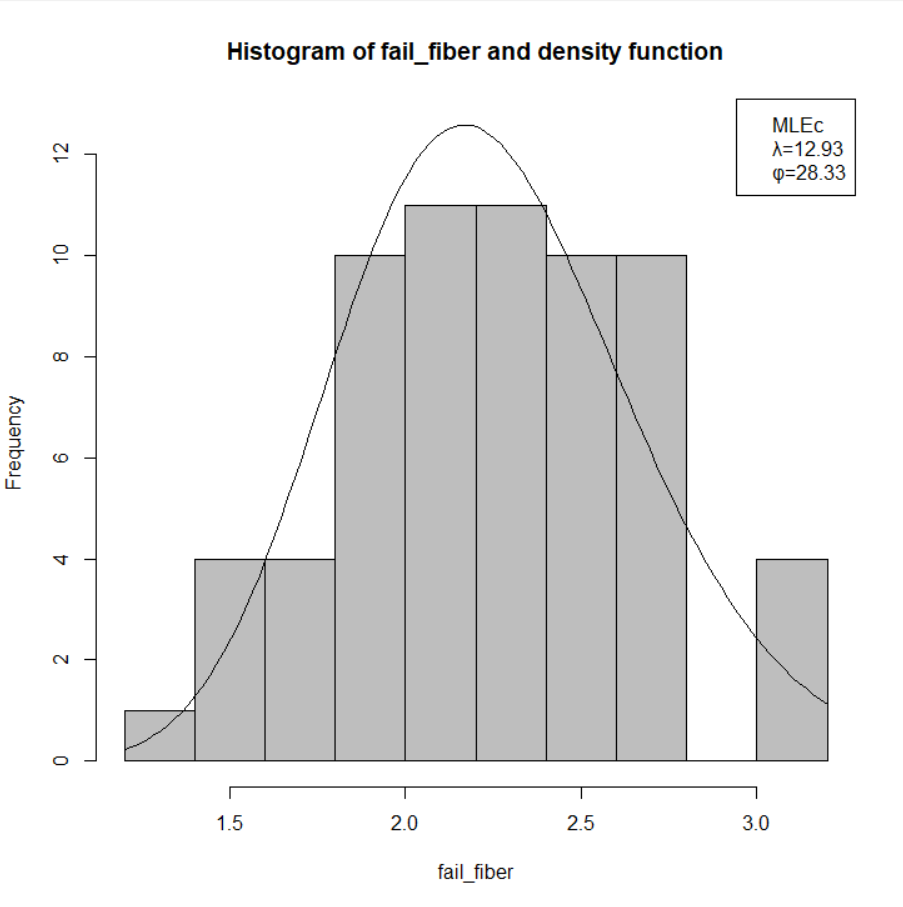
\includegraphics[width=6.5cm,clip]{hist2.png}
		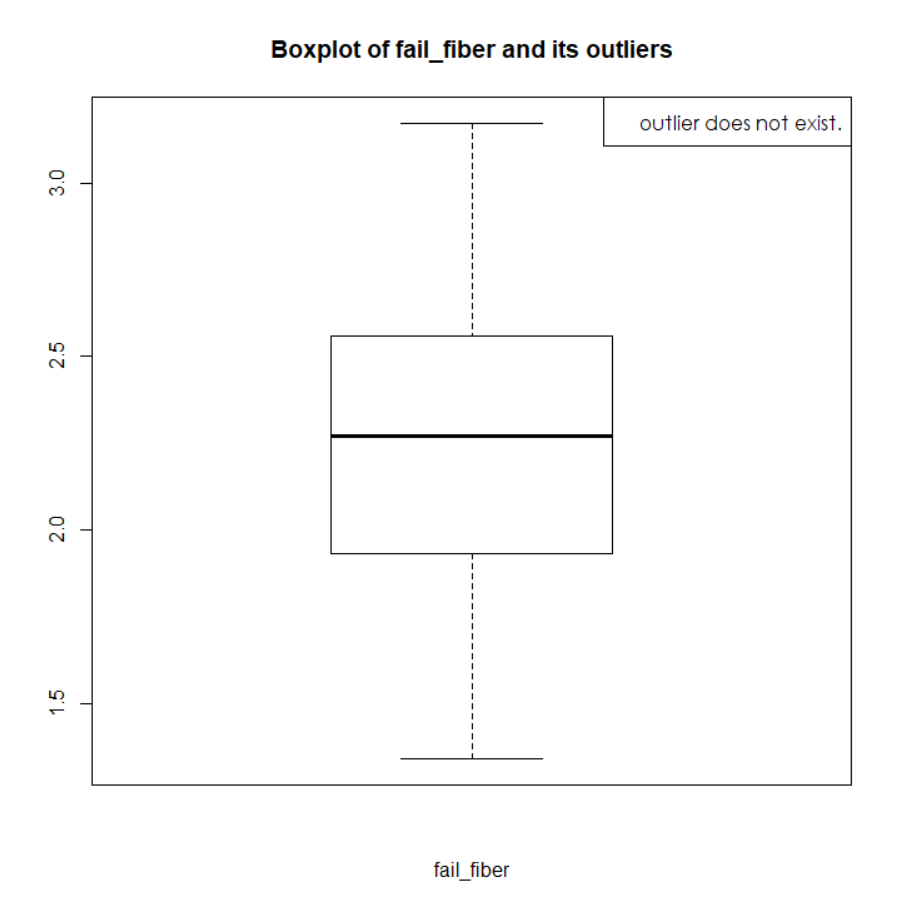
\includegraphics[width=6.5cm,clip]{boxplot2.png}
		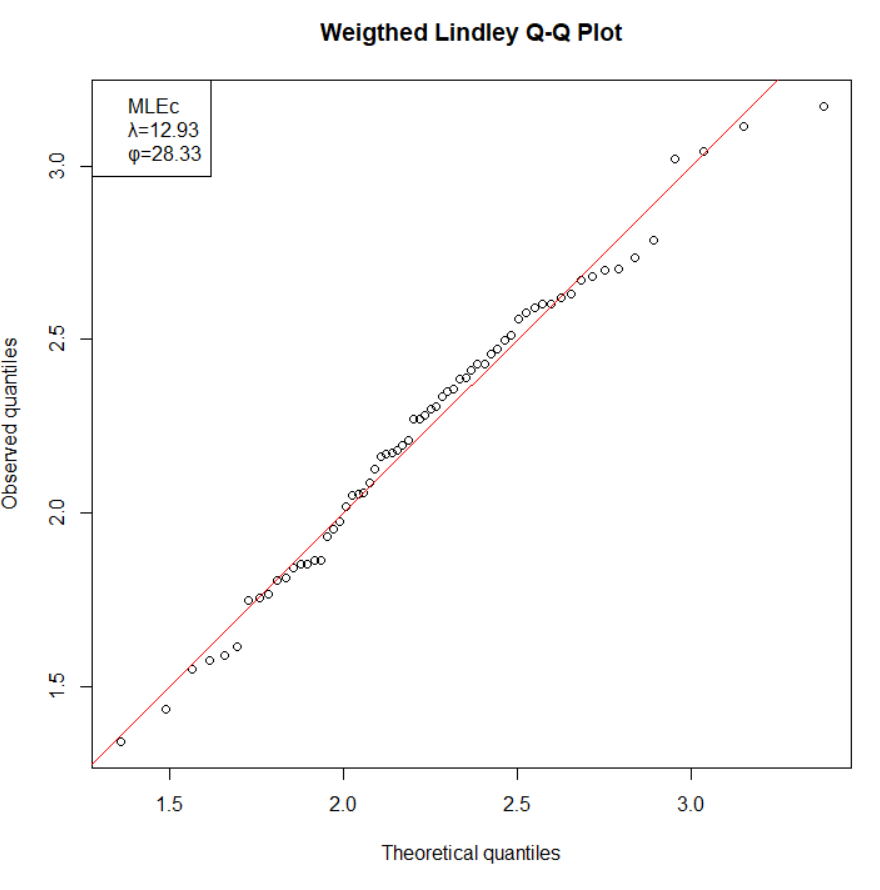
\includegraphics[width=6.5cm,clip]{qq2.png}
		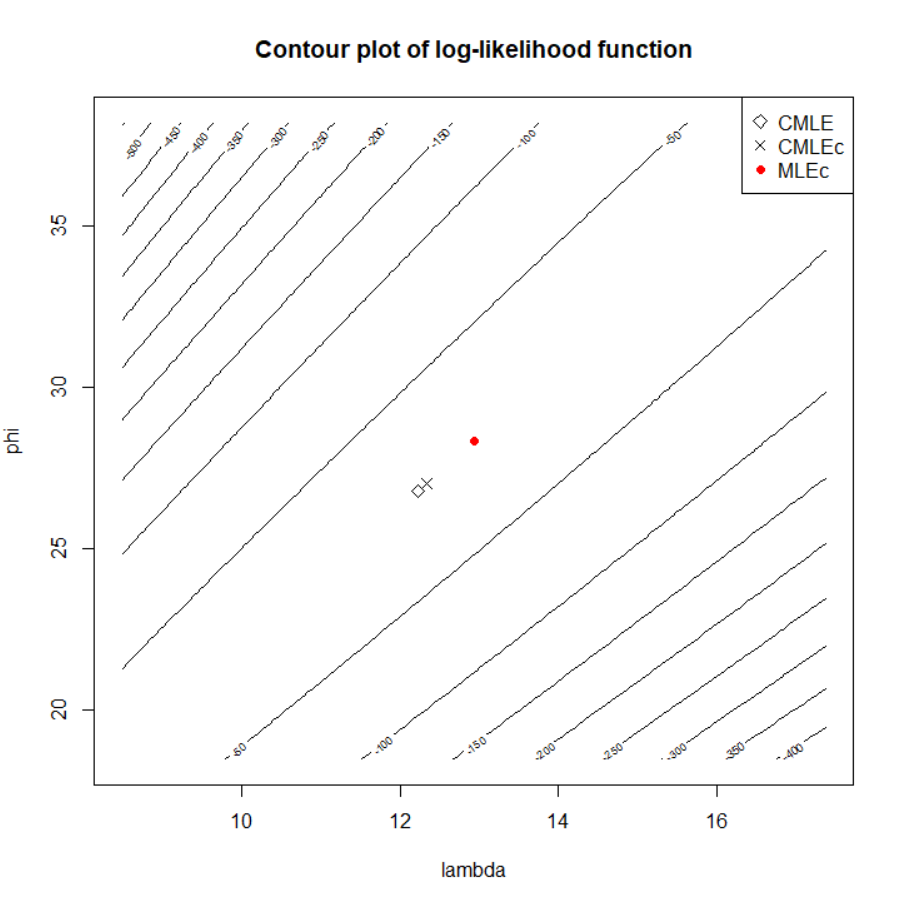
\includegraphics[width=6.5cm,clip]{contour2.png}
		\caption{Histogram with estimated density function, boxplot for detecting outliers, weighted Lindley QQ plot, and contour plot of log-likelihood function with point estimates for a real data fail\_fiber.}  	\label{fig:histogram}
	\end{center}
\end{figure}

To obtain some helpful plots, we use \code{plot} function. Four plots are returned by \code{plot(fiber)} as per Figure \ref{fig:histogram}: the histogram with estimated density function, the boxplot for detecting outliers, QQ plot, and contour plot with point estimates. The first three plots provide insight on how much WL distribution is suitable for the given data, along with the goodness of fit tests. The last contour plot provides the surface of log likelihood near point estimates. Note that the density function in the histogram and the quantiles for the QQ plot are calculated based on estimated parameters.





\section{Summary}
We presented an R package \pkg{WLinfer} that implements a goodness of fit test, several types of point estimation, bias correction, interval estimation, and the likelihood ratio test, and provide some useful plots. We supply a set of simple codes and an illustrative example of how to apply this package in practice. This package could practically assist practitioners, removing the need to make codes from scratch. 






\section{Acknowledgments}

%This paper was written as part of Konkuk University's research support program for its faculty on sabbatical leave in 2020.
%This paper was supported by Konkuk University in 2018.
%The corresponding author's research was supported by Basic Science Research Program through the National Research Foundation of Korea(NRF) funded by the Ministry of Education (2018R1D1A1B07045603).
The corresponding author's research was supported by the Basic Science Research Program through the National Research Foundation of Korea (NRF) funded by the Ministry of Education(2018R1D1A1B07045603) and a National Research Foundation of Korea (NRF) grant funded by the Korean government (MSIT) (2021R1A4A5032622).

\bibliography{Rjreferences}



\address{Yu-Hyeong Jang\\
	Department of Statistics\\
	Korea University\\
	Seoul, Republic of Korea\\
	\email{jyhmaru@gmail.com}}

\address{SungBum Kim\\
	Department of Applied Statistics\\
	Konkuk University\\
	Seoul, Republic of Korea\\
	\email{kimsb0707@hanmail.net}}

\address{Hyun-Ju Jung\\
	Department of Applied Statistics\\
	Konkuk University\\
	Seoul, Republic of Korea\\
	\email{jhjstat@hanmail.net}}

\address{Hyoung-Moon Kim (Corresponding author)\\
	Department of Applied Statistics\\
	Konkuk University\\
	Seoul, Republic of Korea\\
	(https://orcid.org/0000-0002-6014-5207)\\
	\email{hmkim@konkuk.ac.kr}}

